% One PE lane (itmn_m2/src/mamba/Mamba_PE_v2.v): register stages A, M, B1, B2, C.
\documentclass[tikz,border=4pt]{standalone}
% Shared style of the RTL diagrams. Build one with: tectonic fig_x.tex
\usepackage{tikz}
\usetikzlibrary{arrows.meta,positioning,fit,calc,backgrounds,shapes.geometric}
\usepackage[T1]{fontenc}
\usepackage{lmodern}
% opaque background, so the SVGs stay readable on dark pages
\tikzset{every picture/.append style={show background rectangle,
         background rectangle/.style={fill=white, draw=none}, inner frame sep=2pt}}
\definecolor{inkA}{HTML}{0B0B0B}
\definecolor{inkB}{HTML}{52514E}
\definecolor{rule}{HTML}{C3C2B7}
\definecolor{fillA}{HTML}{F0EFEC}
\definecolor{fillPE}{HTML}{CDE2FB}
\definecolor{fillRow}{HTML}{FBE0D3}
\definecolor{fillMem}{HTML}{E5F4EC}
\definecolor{fillCtl}{HTML}{FDF0C8}
\definecolor{fillReg}{HTML}{F6C9A8}
\definecolor{ctlink}{HTML}{8A6A00}
\tikzset{
  blk/.style={draw=inkB, line width=0.5pt, rounded corners=1.5pt, align=center, font=\scriptsize, inner sep=2pt},
  pe/.style={blk, fill=fillPE},
  row/.style={blk, fill=fillRow},
  mem/.style={blk, fill=fillMem},
  ctl/.style={blk, fill=fillCtl},
  plain/.style={blk, fill=white},
  grp/.style={draw=rule, line width=0.6pt, rounded corners=3pt, inner sep=4pt},
  dgrp/.style={draw=inkB, dashed, line width=0.5pt, rounded corners=3pt, inner sep=4pt},
  arr/.style={-{Stealth[length=3pt]}, line width=0.5pt, draw=inkB},
  darr/.style={{Stealth[length=3pt]}-{Stealth[length=3pt]}, line width=0.5pt, draw=inkB},
  carr/.style={-{Stealth[length=2.5pt]}, line width=0.4pt, draw=ctlink, densely dashed},
  lbl/.style={font=\scriptsize, text=inkB, align=center},
  tlbl/.style={font=\tiny, text=inkB, align=center},
  clbl/.style={font=\tiny, text=ctlink, align=center},
  opc/.style={circle, draw=inkB, fill=white, line width=0.5pt, minimum size=0.42cm, inner sep=0pt, font=\scriptsize},
  mux/.style={trapezium, trapezium stretches=true, trapezium angle=70, draw=inkB, fill=fillA, line width=0.5pt, minimum height=0.38cm,
              inner sep=1pt, font=\tiny, shape border rotate=180},
  regbar/.style={draw=inkB, fill=fillReg, line width=0.5pt, minimum height=0.16cm, inner sep=0pt},
}
% bus width mark: \bw{coordinate}{width}
\newcommand{\bw}[2]{\draw[line width=0.4pt, draw=inkB] ($(#1)+(-0.06,-0.06)$) -- ($(#1)+(0.06,0.06)$)
  node[tlbl, anchor=west, inner sep=1pt] {#2};}

\begin{document}
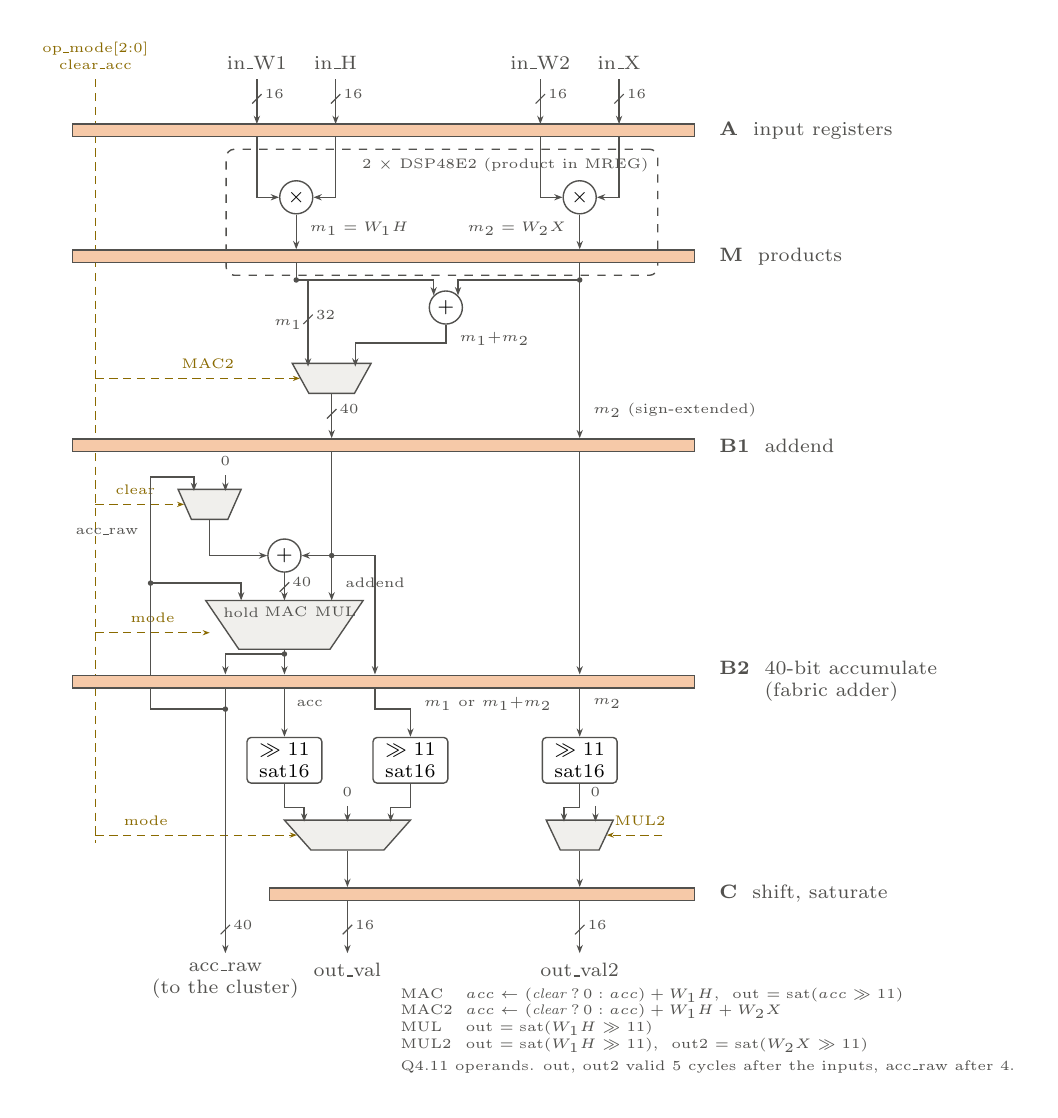
\begin{tikzpicture}[x=1cm,y=1cm]
  % ---------------------------------------------------------------- inputs
  \node[clbl, anchor=south] at (0.55,10.65) {op\_mode[2:0]\\clear\_acc};
  \foreach \n/\x in {in\_W1/2.6, in\_H/3.6, in\_W2/6.2, in\_X/7.2} {\node[lbl, anchor=south] at (\x,10.65) {\n};}
  \foreach \x in {2.6, 3.6, 6.2, 7.2} {\draw[arr] (\x,10.65) -- (\x,10.08); \bw{\x,10.4}{16}}
  % control pipeline (registered with the data in every stage)
  \draw[carr, -] (0.55,10.65) -- (0.55,0.95);

  % ---------------------------------------------------------------- stage M: two DSP48E2 multipliers
  \node[opc] (m1) at (3.1,9.15) {$\times$};
  \node[opc] (m2) at (6.7,9.15) {$\times$};
  \draw[arr] (2.6,9.92) |- (m1.west);
  \draw[arr] (3.6,9.92) |- (m1.east);
  \draw[arr] (6.2,9.92) |- (m2.west);
  \draw[arr] (7.2,9.92) |- (m2.east);
  \draw[arr] (m1.south) -- (3.1,8.49);
  \draw[arr] (m2.south) -- (6.7,8.49);
  \node[tlbl, anchor=west] at (3.15,8.75) {$m_1 = W_1 H$};
  \node[tlbl, anchor=east] at (6.65,8.75) {$m_2 = W_2 X$};
  \node[dgrp, fit={(2.35,9.62) (7.55,8.3)}] (dsp) {};
  \node[tlbl, anchor=north east] at (dsp.north east) {2 $\times$ DSP48E2 (product in MREG)};

  % ---------------------------------------------------------------- stage B1: addend select
  \node[opc] (s12) at (5.0,7.75) {$+$};
  \draw[arr] (3.1,8.32) -- (3.1,8.1) -| (s12.north west);
  \draw[arr] (6.7,8.32) -- (6.7,8.1) -| (s12.north east);
  \node[mux, minimum width=1.0cm] (amx) at (3.55,6.85) {};
  \draw[arr] (3.1,8.1) -- (3.25,8.1) -- (3.25,7.0);
  \draw[arr] (s12.south) |- (4.4,7.3) -| (3.85,7.0);
  \node[tlbl, anchor=south] at (3.0,7.35) {$m_1$};
  \node[tlbl, anchor=west] at (5.05,7.35) {$m_1{+}m_2$};
  \draw[carr] (0.55,6.85) -- (amx.west) node[clbl, pos=0.55, above] {MAC2};
  \draw[arr] (amx.south) -- (3.55,6.09);
  \draw[arr] (6.7,8.1) -- (6.7,6.09);
  \node[tlbl, anchor=west] at (6.75,6.45) {$m_2$ (sign-extended)};
  \bw{3.25,7.6}{32}
  \bw{3.55,6.4}{40}

  % ---------------------------------------------------------------- stage B2: accumulate in the fabric
  % clear mux: 0 or acc_raw
  \node[mux, minimum width=0.8cm] (cmx) at (2.0,5.25) {};
  \node[tlbl, anchor=south] (z1) at (2.2,5.62) {0};
  \draw[arr] (z1.south) -- (2.2,5.42);
  \node[opc] (acc) at (2.95,4.6) {$+$};
  \draw[arr] (cmx.south) |- (acc.west);
  \draw[arr] (3.55,5.91) -- (3.55,4.6) -- (acc.east);
  \draw[carr] (0.55,5.25) -- (cmx.west) node[clbl, pos=0.45, above] {clear};
  % acc_next mux: hold / MAC / load
  \node[mux, minimum width=2.0cm, minimum height=0.62cm] (nmx) at (2.95,3.72) {};
  \draw[arr] (acc.south) -- (2.95,4.03);
  \draw[arr] (3.55,4.6) -- (3.55,4.03);
  \node[tlbl] at (2.4,3.88) {hold};
  \node[tlbl] at (2.97,3.88) {MAC};
  \node[tlbl] at (3.6,3.88) {MUL};
  \draw[carr] (0.55,3.62) -- (2.0,3.62) node[clbl, pos=0.5, above] {mode};
  \node[tlbl, anchor=west] at (3.6,4.25) {addend};
  % next value -> acc_raw and acc_sat_src
  \draw[arr] (nmx.south) -- (2.95,3.09);
  \draw[arr] (2.95,3.35) -- (2.2,3.35) -- (2.2,3.09);
  % mul sources
  \draw[arr] (3.55,4.6) -- (4.1,4.6) -- (4.1,3.09);
  \draw[arr] (6.7,5.91) -- (6.7,3.09);
  % feedback acc_raw
  \draw[arr] (2.2,2.91) -- (2.2,2.65) -- (1.25,2.65) -- (1.25,5.6) -| (1.8,5.42);
  \draw[arr] (1.25,4.25) -| (2.4,4.03);
  \fill[inkB] (1.25,4.25) circle (0.035) (2.2,2.65) circle (0.035) (3.55,4.6) circle (0.035) (2.95,3.35) circle (0.035);
  \fill[inkB] (3.1,8.1) circle (0.035) (6.7,8.1) circle (0.035);
  \node[tlbl, anchor=east] at (1.22,4.9) {acc\_raw};
  \bw{2.95,4.2}{40}

  % ---------------------------------------------------------------- stage C: shift, saturate, select
  \node[plain, minimum width=0.95cm] (sh1) at (2.95,2.0) {$\gg 11$\\sat16};
  \node[plain, minimum width=0.95cm] (sh2) at (4.55,2.0) {$\gg 11$\\sat16};
  \node[plain, minimum width=0.95cm] (sh3) at (6.7,2.0) {$\gg 11$\\sat16};
  \draw[arr] (2.95,2.91) -- (sh1.north);
  \draw[arr] (4.1,2.91) -- (4.1,2.65) -| (sh2.north);
  \draw[arr] (6.7,2.91) -- (sh3.north);
  \node[tlbl, anchor=west] at (2.98,2.72) {acc};
  \node[tlbl, anchor=west] at (4.6,2.72) {$m_1$ or $m_1{+}m_2$};
  \node[tlbl, anchor=west] at (6.75,2.72) {$m_2$};
  \node[mux, minimum width=1.6cm] (omx) at (3.75,1.05) {};
  \draw[arr] (sh1.south) -- (2.95,1.4) -| (3.2,1.22);
  \draw[arr] (sh2.south) -- (4.55,1.4) -| (4.3,1.22);
  \node[tlbl, anchor=south] (z2) at (3.75,1.42) {0};
  \draw[arr] (z2.south) -- (3.75,1.22);
  \draw[carr] (0.55,1.05) -- (omx.west) node[clbl, pos=0.25, above] {mode};
  \node[mux, minimum width=0.85cm] (o2mx) at (6.7,1.05) {};
  \draw[arr] (sh3.south) -- (6.7,1.4) -| (6.5,1.22);
  \node[tlbl, anchor=south] (z3) at (6.9,1.42) {0};
  \draw[arr] (z3.south) -- (6.9,1.22);
  \draw[carr] (7.75,1.05) -- (o2mx.east) node[clbl, pos=0.4, above] {MUL2};
  \draw[arr] (omx.south) -- (3.75,0.39);
  \draw[arr] (o2mx.south) -- (6.7,0.39);

  % ---------------------------------------------------------------- outputs
  \draw[arr] (3.75,0.21) -- (3.75,-0.45) node[lbl, anchor=north] {out\_val};
  \draw[arr] (6.7,0.21) -- (6.7,-0.45) node[lbl, anchor=north] {out\_val2};
  \draw[arr] (2.2,2.65) -- (2.2,-0.45) node[lbl, anchor=north, align=center] {acc\_raw\\(to the cluster)};
  \bw{3.75,-0.15}{16}
  \bw{6.7,-0.15}{16}
  \bw{2.2,-0.15}{40}

  % ---------------------------------------------------------------- register stages, drawn over the wires
  \foreach \y in {10.0, 8.4, 6.0, 3.0} {\node[regbar, minimum width=7.9cm, anchor=west] at (0.25,\y) {};}
  \node[regbar, minimum width=5.4cm, anchor=west] at (2.75,0.3) {};
  \node[lbl, anchor=west, align=left] at (8.35,10.0) {\textbf{A}\ \ input registers};
  \node[lbl, anchor=west, align=left] at (8.35,8.4) {\textbf{M}\ \ products};
  \node[lbl, anchor=west, align=left] at (8.35,6.0) {\textbf{B1}\ \ addend};
  \node[lbl, anchor=west, align=left] at (8.35,3.0) {\textbf{B2}\ \ 40-bit accumulate\\\phantom{\textbf{B2}}\ \ (fabric adder)};
  \node[lbl, anchor=west, align=left] at (8.35,0.3) {\textbf{C}\ \ shift, saturate};

  % ---------------------------------------------------------------- modes
  \node[tlbl, anchor=north west, align=left] at (4.3,-0.75) {%
    \begin{tabular}{@{}l@{\ \ }l@{}}
    MAC  & $acc \leftarrow (\mathit{clear}\,?\,0 : acc) + W_1 H$, \ out $= \mathrm{sat}(acc \gg 11)$ \\
    MAC2 & $acc \leftarrow (\mathit{clear}\,?\,0 : acc) + W_1 H + W_2 X$ \\
    MUL  & out $= \mathrm{sat}(W_1 H \gg 11)$ \\
    MUL2 & out $= \mathrm{sat}(W_1 H \gg 11)$, \ out2 $= \mathrm{sat}(W_2 X \gg 11)$ \\[2pt]
    \multicolumn{2}{@{}l@{}}{Q4.11 operands. out, out2 valid 5 cycles after the inputs, acc\_raw after 4.}
    \end{tabular}};
\end{tikzpicture}
\end{document}
